
\documentclass[conference]{IEEEtran}
\usepackage{graphicx,times,amsmath,colortbl, psfrag} % Add all your packages here

\usepackage[ruled, vlined, english, boxed, linesnumbered, lined]{algorithm2e}
%\renewcommand{\algorithmicrequire}{\textbf{Input:}}
%\renewcommand{\algorithmicensure}{\textbf{Output:}}
\usepackage{algpseudocode} 

\usepackage{multirow}

\usepackage {amsfonts}
\usepackage {amsmath}




% *** GRAPHICS RELATED PACKAGES ***
%\usepackage[pdftex]{graphicx}
%%
%\ifCLASSINFOpdf
%   
%  % declare the path(s) where your graphic files are
%   \graphicspath{{../pdf/}{../jpeg/}}
%  % and their extensions so you won't have to specify these with
%  % every instance of \includegraphics
%   \DeclareGraphicsExtensions{.pdf,.jpeg,.png}
%\else
%  \fi


\begin{document}
%
% paper title
% can use linebreaks \\ within to get better formatting as desired
\title{Pr\'actica 1. ``An\'alisis experimental de la eficiencia de algoritmos de ordenamiento''}


% author names and affiliations
% use a multiple column layout for up to three different
% affiliations
\author{\IEEEauthorblockN{Christian Miguel Hern\'andez Mej\'ia}

\IEEEauthorblockA{
Departamento de Ciencias e Ingenier\'ia de la Computaci\'on,\\ 
An\'alisis de Algoritmos, ESCOM-IPN\\
 (email: christian.mhm@outlook.com)
}
}
% make the title area
\maketitle



\section{Objetivo}
El alumno realizar\'a un an\'alisis a posteriori de diversos algoritmos de ordenamiento. Implementar\'a y comparar\'a la eficiencia de estos algoritmos en los casos mejor, peor y promedio.

\section{Intrucciones}

Para mostrar la eficiencia de diferentes algoritmos que solucionan un mismo problema, se consider\'o el problema de ordenamiento de una lista de n\'umeros enteros. Los algoritmos que se implementar\'an son:

\begin{enumerate}
	\item Ordenamiento por inseci\'on
	\item El m\'etodo de la burbuja 
	\item Ordenamiento por mezcla
	\item Ordenamiento r\'apido (Quick-sort)
\end{enumerate}

Considere como entrada, conjuntos de n\'umeros enteros con $\{100, 200, 300, \ldots, 10,000\}$ elementos.
Deber\'a realizar la ejecuci\'on de cada algoritmo para el mejor y peor caso. Adem\'as debe usar los datos de entrada proporcionados por el profesor para el caso promedio.
Deber\'a reportar el tiempo de ejecuci\'on (en segundos) de cada instancia  como se pide en la Tabla 1.
Una vez que se tengan los datos del tiempo de ejecuci\'on grafique (de preferencia en python o gnuplot) estos resultados (ver ejemplo en Figura 1).

Deber\'a enviar al correo \href{miriam.pescador@gmail.com}, una carpeta comprimida con la implementaci\'on de los c\'odigos python y el reporte en formato latex y pdf.
El asunto del correo deber\'a decir "Practica 1 Analisis de Algoritmos [nombre completo del alumno comenzando con el apellido paterno]".
La carpeta debe tener el nombre del alumno (comenzando por apellido paterno).
La fecha l\'imite de entrega es el pr\'oximo Martes 5 de febrero de 2019 a las 10:00 pm. Por cada d\'ia de retraso se penalizar\'a al alumno con 15\% de la calificaci\'on obtenida. 

El reporte en latex debe considerar las siguientes secciones:

\begin{itemize}
\item Introducci\'on: descripci\'on sobre la implementaci\'on de la pr\'actica
\item Marco te\'orico. En esta secci\'on deber\'a poner los conceptos de:
\begin{itemize}
	\item Algoritmo
	\item An\'alisis a priori y posteriori
	\item An\'alisis del mejor y peor caso
	\item Caso promedio
\end{itemize}
Incluya la bibliograf\'ia que fue consultada (use el formato de ejemplo para agregarlo a su reporte).
\item Implementaci\'on. Coloque en esta secci\'on los algoritmos proporcionados en la plantilla de latex. Proporcione informaci\'on sobre las caracter\'isticas del equipo de c\'omputo donde realiz\'o las pruebas (sistema operativo, tipo de procesador, memoria, etc.).
Adem\'as deber\'a documentar las bibliotecas que empleo para la implementaci\'on de los algoritmos.
\item Resultados. Incluya la tabla de resultados y graficas solicitadas.
\item Conclusiones. Describa cu\'ales fueron los mejores algoritmos y para qu\'e casos y/o n\'umero de datos de entrada. Proporcione una justificaci\'on del por qu\'e se obtuvieron estos resultados. 
\end{itemize} 

\subsection{Algoritmos}

\begin{algorithm}[h]
%\hspace*{\algorithmicindent} \textbf{Input.} {A: conjunto de n\'umeros enteros} \\
%\hspace*{\algorithmicindent} \textbf{Output.} {A: lista ordenada de los n\'umeros enteros}
\KwData{A : list of sortable items}
\Begin{	
  InsertionSort(A){ \\
  
	\For{$ i \leftarrow 2$ to $n$}{
		$j \leftarrow   i - 1 $;\\
		\While{$j \geq 1 $ and $A[j] > A[j+1]$}{
			swap(A[j], A[j+1]);\\
			$j \leftarrow j-1$;\\		
		}
	}
	return A;	
}
}
\caption{Insertion Sort Algorithm}
\label{merge}
\end{algorithm}

\begin{algorithm}[h]
%\Begin{	
  MergeSort(A, $p$, $r$){ \\
  
	\If{$p < r$}{
		$q \leftarrow   \lfloor (p+r)/2 \rfloor $;\\
		MergeSort(A, $p$, $q$);\\
		MergeSort(A, $q+1$, $r$);\\
		Merge(A, $p$, $q$, $r$);
	}
	return A;	
%}
}
\caption{Merge Sort Algorithm}
\label{merge}
\end{algorithm}
 

\begin{algorithm}[h]
\KwData{A : list of sortable items}
\Begin{	
  $n \leftarrow length(A)$;\\
   \Repeat{not swapped}{
      $swapped \leftarrow false$;\\
      \For { $i \leftarrow 1$ to $n$}{
           \If {$A[i-1] > A[i]$} {
            swap(A[i-1], A[i]);\\
            $swapped \leftarrow true$;\\
            }
      }
      $n \leftarrow n - 1$;
   } 
   return A;	
}
\caption{Bubble Sort Algorithm}
\label{bubble}
\end{algorithm}
 

\begin{algorithm}[h]
%\Begin{	
  QuickSort(A, $p$, $r$){ \\
	\If{$p < r$}{
		$q \leftarrow   Partition(A, p, r)$;\\
		QuickSort(A, $p$, $q$);\\
		QuickSort(A, $q+1$, $r$);\\
		
	}
	return A;	
%}
}
\caption{Quick Sort Algorithm}
\label{quick}
\end{algorithm}


\begin{algorithm}[h]
%\Begin{	
 Partition(A, $p$, $r$){ \\
  $x \leftarrow A[p]$;\\
  $i \leftarrow p-1$
  $j \leftarrow r+1$
  \While{true}{
   	\Repeat{$A[j]\leq x$}{
      		$j \leftarrow j - 1$;\\
	 }
	 \Repeat{$A[j]\geq x$}{
      		$i \leftarrow i + 1$;\\
	 }
	 \If{i < j}{
	 	exchange $A[i] \leftrightarrow A[j] $;
	 }
	 \Else{return j;}
      		
    }	
}
\caption{Partition Algorithm}
\label{partition}
\end{algorithm}



La figura \ref{fig:grafica} muestra el comportamiento de las funciones.

\begin{figure}
	\centering
	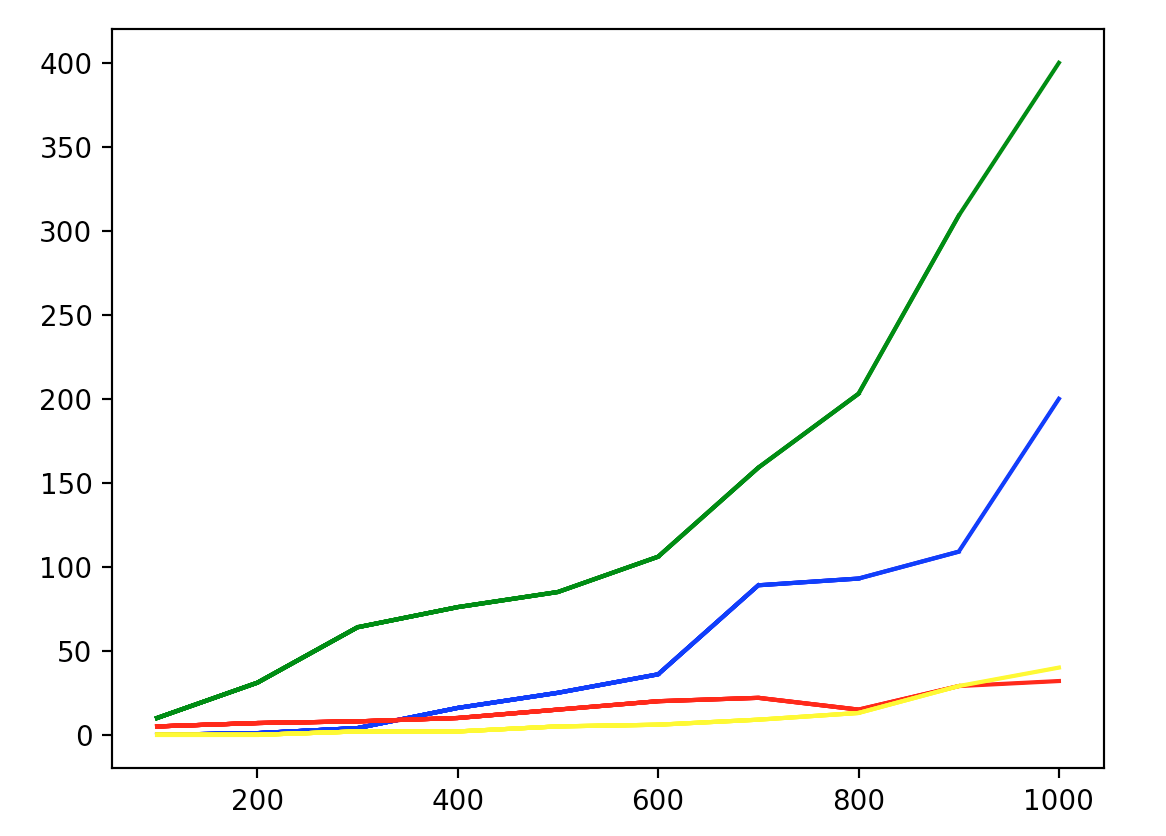
\includegraphics[width=1.0\columnwidth]{Imagenes/grafica1.png}
	\caption{Comparaci\'on del comportamiento de los algoritmos}
	\label{fig:grafica}
\end{figure}

%%%%%%%%%%%%%%%%%%%%%%%%%%%%%%%%%%%%%%%%%%%%%%%%%
\begin{table*}[!ht]
\begin{tabular}{|c|c|c|c|c|c|c|c|c|c|c|c|c|}
\hline
\multirow{2}{*}{n} & \multicolumn{4}{c|}{Mejor Caso} & \multicolumn{4}{c|}{Peor Caso} & \multicolumn{4}{c|}{Caso promedio} \\ 
\cline{2-13}
& insertion & merge & bubble & quick-sort & insertion & merge & bubble & quick-sort & insertion & merge & bubble & quick-sort \\ 
\hline
100 & 0.00004 & 0.00051 & 0.00002 & 0.00041 & 0.0051 & 0.00072 & 0.00451 & 0.00138 &0.00269 & 0.00073 & 0.00302 & 0.0005 \\
\hline
200 & 0.00007 & 0.00119 & 0.00004 & 0.0008 & 0.01916 & 0.00142 & 0.01697 & 0.00493 &0.00992 & 0.00144 & 0.01065 & 0.00109 \\
\hline
300 & 0.00012 & 0.00177 & 0.00006 & 0.00123 & 0.0445 & 0.00214 & 0.03682 & 0.00961 &0.02035 & 0.0022 & 0.02188 & 0.0015 \\
\hline
400 & 0.00015 & 0.00236 & 0.00008 & 0.00189 & 0.07573 & 0.00304 & 0.06223 & 0.01633 &0.0357 & 0.00273 & 0.03949 & 0.00208 \\
\hline
500 & 0.00021 & 0.00309 & 0.00011 & 0.00223 & 0.11081 & 0.00303 & 0.09037 & 0.0257 &0.05057 & 0.00324 & 0.05765 & 0.00252 \\
\hline
600 & 0.00024 & 0.00387 & 0.00014 & 0.00285 & 0.15409 & 0.00399 & 0.13395 & 0.03691 &0.07657 & 0.00415 & 0.08583 & 0.00337 \\
\hline
700 & 0.0003 & 0.00457 & 0.00016 & 0.00346 & 0.22882 & 0.00506 & 0.18777 & 0.05388 &0.11413 & 0.00496 & 0.12575 & 0.00476 \\
\hline
800 & 0.00034 & 0.00528 & 0.00019 & 0.00405 & 0.32366 & 0.00631 & 0.26037 & 0.06509 &0.14958 & 0.00547 & 0.16437 & 0.00491 \\
\hline
900 & 0.00038 & 0.0059 & 0.00021 & 0.00456 & 0.37904 & 0.00647 & 0.30892 & 0.07697 &0.20877 & 0.00615 & 0.20181 & 0.00495 \\
\hline
1000 & 0.00043 & 0.00665 & 0.00024 & 0.00493 & 0.47107 & 0.00787 & 0.45145 & 0.11483 &0.227 & 0.00683 & 0.25352 & 0.00568 \\
\hline
1100 & 0.00049 & 0.0077 & 0.00028 & 0.00574 & 0.60479 & 0.00821 & 0.53072 & 0.12596 &0.29485 & 0.00762 & 0.31975 & 0.00652 \\
\hline
1200 & 0.00052 & 0.00833 & 0.00029 & 0.00623 & 0.73021 & 0.012 & 0.64184 & 0.17054 &0.35064 & 0.00859 & 0.37459 & 0.00726 \\
\hline
1300 & 0.00059 & 0.00919 & 0.00034 & 0.00718 & 0.80978 & 0.00976 & 0.72414 & 0.17043 &0.41011 & 0.00942 & 0.42794 & 0.00766 \\
\hline
1400 & 0.0006 & 0.00986 & 0.00038 & 0.00805 & 1.00332 & 0.00999 & 0.86745 & 0.19028 &0.46963 & 0.0097 & 0.51216 & 0.00835 \\
\hline
1500 & 0.00058 & 0.01049 & 0.00039 & 0.00882 & 1.15588 & 0.01163 & 0.928 & 0.21852 &0.52731 & 0.01053 & 0.58435 & 0.00964 \\
\hline
1600 & 0.00069 & 0.01135 & 0.00042 & 0.00923 & 1.24741 & 0.01139 & 1.01678 & 0.24528 &0.63197 & 0.01191 & 0.65451 & 0.00968 \\
\hline
1700 & 0.00076 & 0.01272 & 0.00048 & 0.01011 & 1.6366 & 0.01329 & 1.12716 & 0.27465 &0.7209 & 0.01262 & 0.75385 & 0.01022 \\
\hline
1800 & 0.00082 & 0.01285 & 0.00047 & 0.01014 & 1.50069 & 0.01236 & 1.22014 & 0.30347 &0.80239 & 0.01377 & 0.84367 & 0.01075 \\
\hline
1900 & 0.00084 & 0.01461 & 0.00048 & 0.0103 & 1.7747 & 0.01406 & 1.43062 & 0.34033 &0.87809 & 0.0142 & 0.99564 & 0.01197 \\
\hline
2000 & 0.00077 & 0.01474 & 0.00055 & 0.01159 & 1.91349 & 0.01463 & 1.71074 & 0.40753 &1.02944 & 0.01859 & 1.22941 & 0.01654 \\
\hline
2100 & 0.00094 & 0.01559 & 0.00059 & 0.01173 & 2.13514 & 0.01541 & 1.81542 & 0.43846 &1.02876 & 0.01565 & 1.14635 & 0.01275 \\
\hline
2200 & 0.00098 & 0.01625 & 0.00061 & 0.01214 & 2.30065 & 0.01619 & 1.95848 & 0.46913 &1.20191 & 0.01673 & 1.30875 & 0.01391 \\
\hline
2300 & 0.00103 & 0.01701 & 0.00064 & 0.01301 & 2.66175 & 0.02212 & 2.30951 & 0.54539 &1.31769 & 0.01752 & 1.42972 & 0.01465 \\
\hline
2400 & 0.00106 & 0.01696 & 0.00059 & 0.01387 & 2.94397 & 0.02053 & 2.46941 & 0.59705 &1.6125 & 0.02102 & 1.61563 & 0.01539 \\
\hline
2500 & 0.00112 & 0.01854 & 0.0007 & 0.0145 & 3.09781 & 0.01917 & 2.63058 & 0.6382 &1.51991 & 0.02061 & 1.70267 & 0.01712 \\
\hline
2600 & 0.00118 & 0.0191 & 0.00062 & 0.01502 & 3.39612 & 0.01877 & 2.7743 & 0.74055 &1.64607 & 0.02099 & 1.84184 & 0.01689 \\
\hline
2700 & 0.00116 & 0.02014 & 0.00071 & 0.01621 & 3.73651 & 0.02184 & 3.05087 & 0.72472 &1.72787 & 0.02079 & 1.87635 & 0.01702 \\
\hline
2800 & 0.00126 & 0.02049 & 0.00067 & 0.01682 & 3.98676 & 0.02571 & 3.29633 & 0.83525 &1.97331 & 0.02183 & 2.35468 & 0.02058 \\
\hline
2900 & 0.00131 & 0.02073 & 0.00073 & 0.01774 & 4.1186 & 0.02124 & 3.23006 & 0.77287 &2.30956 & 0.02337 & 2.29632 & 0.01913 \\
\hline
3000 & 0.00121 & 0.02196 & 0.00075 & 0.01807 & 4.36995 & 0.0224 & 3.51441 & 0.88998 &2.15485 & 0.02522 & 2.33197 & 0.02223 \\
\hline

\end{tabular}
\caption{Resultados de los tiempos de ejecuci\'on para cada algoritmo.}
\end{table*}


%\bibliography{my-paper}


% (used to reserve space for the reference number labels box)
\begin{thebibliography}{1}

\bibitem{moscato99}
P. Moscato,
\newblock {\em On evolution, search, optimization, genetic algorithms and martial arts: Towards memetic algorithms,}
\newblock  Technical Report C3P Report 826, 1989.

\bibitem{KrasnogorS00}%
N. Krasnogor and J. Smith,
\newblock {\em A Memetic Algorithm With Self-Adaptive Local Search: TSP as a case study,}
\newblock Genetic Evolutionary Computation Conference pp. 987-994, 2000. 

\end{thebibliography}

\end{document}


